%%%%%%%%%%%%%%%%%%%%%%%%%%%%% Define Article %%%%%%%%%%%%%%%%%%%%%%%%%%%%%%%%%%
\documentclass{article}
%%%%%%%%%%%%%%%%%%%%%%%%%%%%%%%%%%%%%%%%%%%%%%%%%%%%%%%%%%%%%%%%%%%%%%%%%%%%%%%

%%%%%%%%%%%%%%%%%%%%%%%%%%%%% Using Packages %%%%%%%%%%%%%%%%%%%%%%%%%%%%%%%%%%
\usepackage{listings, xcolor}
\usepackage{parskip}
\usepackage{hyperref}
\usepackage{amsmath}
\usepackage{graphicx}
\usepackage[a4paper, margin = 1.5cm]{geometry}
\usepackage{float}
\usepackage{amsmath}
\usepackage{amssymb}
\usepackage{parskip}
\usepackage{listings}
\usepackage{caption}

\lstset{
frame = shadowbox,
basicstyle = \small\ttfamily,
mathescape = true,
numbers = left,
commentstyle = \itshape\color{gray}
columns = flexible,
keepspaces = true,
moredelim = [l]{//}
}

%%%%%%%%%%%%%%%%%%%%%%%%%%%%%% Title & Author %%%%%%%%%%%%%%%%%%%%%%%%%%%%%%%%
\title{Progettazione Architetturale del SW}
\author{Trentin Tommaso}
%%%%%%%%%%%%%%%%%%%%%%%%%%%%%%%%%%%%%%%%%%%%%%%%%%%%%%%%%%%%%%%%%%%%%%%%%%%%%%
\begin{document}
  \maketitle
  \tableofcontents
  \newpage

  \section{Progettazione del SW}
    La progettazione architetturale si colloca nella fase di Progettazione del sistema ed ha un \textbf{ruolo chiave nello sviluppo}, rappresentando il collegamento critico tra ingegneria dei requisiti e progettazione di dettaglio dei componenti.
    \subsection{Finalità}
      Progettare = seguire un processo di risoluzione mirando a descrivere un modo:
      \begin{itemize}
          \item per implementare requisiti funzionali; 
          \item rispettando vincoli dei requisiti non funzionali; 
          \item in conformità con principi di buona qualità.
      \end{itemize}
    \subsection{Decisioni di progettazione}
      Progettista affronta una sereie di problemi di progettazione, ognuno di questi ha normalmente alcune soluzioni alternative (\textbf{design options}). \\ 
      Progettista effettua una serie di \textbf{design decision} oer risolvere il problema scegliendo la \textit{migliore} alternativa possibile in base a requisiti sistema e background / esperienza architetti. \\
      \noindent
        \begin{minipage}[c]{0.38\linewidth}
            \textbf{Design space}: insieme possibili progetti che saranno implementabili scegliendo tra varie alternative.
        \end{minipage}
        \hfill
        \begin{minipage}[c]{0.58\linewidth}
            \centering
            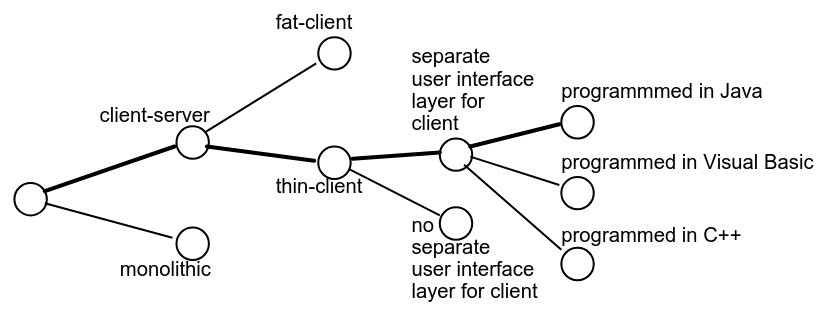
\includegraphics[width=0.8\linewidth]{figures/des_dec.png}
        \end{minipage}
      \subsubsection{Top-Down}
        \begin{itemize}
          \item Si parte da progettazione della struttura ad altissimo livello del sistema, per poi procedere gradualmente più nel dettaglio riguardo aspetti di più basso livello (es. definizione architettura SW e tipo di DB impiegato -> definire formato di dati, algoritmi usati, interfacce utente);
          \item Necessaria per definire una buona struttura per il sistema.
        \end{itemize}
      \subsubsection{Bottom-Up}
        \begin{itemize}
          \item Si parte progettando componenti di basso livello e si decide poi come collegarli per ottenere i componenti di livello più alto; 
          \item Serve a progettare componenti riusabili in altri punti del sistema.
        \end{itemize}
  \section{Progettazione Architetturale}
    Si occupa di comprendere come organizzare il sistema SW e progettarne la sua struttura complessiva, identifica i componenti strutturali di un sistema e le loro relazioni / interfacce; ha come output un modello che descrive l'organizzazione del sistema e la comunicazione tra i suoi componenti.
    \subsection{Architettura, requisiti e prestazioni}
      Architettura SW è importante in quanto influisce (o addirittura pone vincoli) su prestazioni / robustezza / distribuzione / manutenibilità di un sistema. \\ 
      \subsubsection{Requisiti non funzionali e stili architetturali}
        \begin{itemize}
            \item \textbf{Performance}: preferenza per componenti grandi, localizzando operazioni critiche e minimizzando comunicazioni; 
            \item \textbf{Protezione}: utilizzo di architettura a strati, posizionando risorse critiche negli strati interni e ponendo convalide ad ogni strato;
            \item \textbf{Sicurezza funzionale}: concentrazione funzionalità critiche per sicurezza in numero limitato di sottosistemi per fornire meccanismi di protezione riducendo i costi;
            \item \textbf{Disponibilità}: utilizzo di componenti ridondanti e meccanismi per tolleranza ai guasti;
            \item \textbf{Manutenibilità}: utilizzo componenti piccoli facilmente sostituibili / modificabili.
        \end{itemize}
    \subsection{Progettazione architetturale e agilità}
      Attività di progettazione architetturale può scontrarsi con principi agili di \textbf{documentazione minima} e \textbf{refactoring} (possibile rifattorizzare singoli componenti ma per l'intera architettura in quanto ciascun cambiamento può interessare diversi componenti).
    \subsection{Vantaggi progettazione esplicità}
      \begin{itemize}
          \item Fornisce presentazione del sistema ad alto livello che consente confronto tra stakeholders;
          \item Durante progettasione viene analizzata conformità del sistema ai requisiti non funzionali;
          \item Modello può essere riusato per sistemi con requisiti simili.
      \end{itemize}
  \section{Pattern Architetturali}
    \subsection{Concetto di pattern}
      Soluzioni a problemi di progettazione comuni e ricorrenti che si incontrano in applicazioni reali, un pattern architetturale descrive l'organizzazione del sistema che è stata utilizzata in diversi sistemi SW. Vantaggiosi in quanto permettono:
      \begin{itemize}
          \item \textbf{Riuso} di conoscenza ed esperienza di progettazione in quanto problemi sono raramente nuovi e unici;
          \item \textbf{Presentazione e comunicazione} in quanto stabiliscono una terminologia comune e condivisa, forniscono una prospettiva di alto livello del sistema e permettono comprensione / discussione del progetto senza dover gestire troppo presto i dettagli.
      \end{itemize}
    \subsection{Pattern multi-layer}
      Decomposizione \textit{gerarchica} del sistema in un insieme ordinato di layer (sottoinsiemi che forniscono servizi correlati), ogni layer può essere a sua volta stratificato in layer più astratti.
      \begin{figure}[htpb]
          \centering
          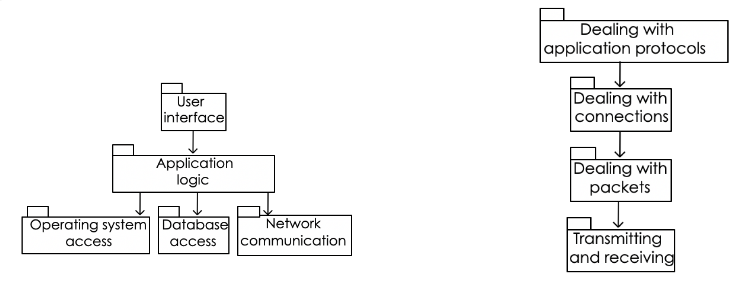
\includegraphics[width=0.8\linewidth]{figures/arch_ml.png}
      \end{figure}
      Fornisce:
      \begin{itemize}
          \item \textbf{separazione}: solitamente elementi che forniscono servizi correlati sono raggruppati nello stesso layer, separati da altri servizi;
          \item \textbf{indipendenza}: possibile progettare uno strato indipendentemente da altri (rispettando le interfacce).
      \end{itemize}
      Grazie a separazione e indipendenza, se si modifica interfaccia / si aggiungono funzionalità ad uno strato, solo strati adiacenti vengono influenzati. Questa è quindi una soluzione ideale per sistemi multipiattaforma (dipendenze della macchina localizzate in strati specifici).
    \subsection{Pattern repository}
      Utilizzato in casi di diversi sottosistemmi con grandi quantità di dati da condividere e memorzzare per molto tempo, questi vengono salvati / gestiti in un database centrale (\textbf{repository}) il cui accesso è consentito a tutti i sottosistemi.
      \begin{itemize}
          \item Tutti i sottosistemi devono operare con un modello dati concordato;
          \item Repo è accessibile a tutti i componenti del sistema;
          \item Componenti scambiano dati solo mediante la repo.
      \end{itemize}
      \begin{figure}[htpb]
          \centering
          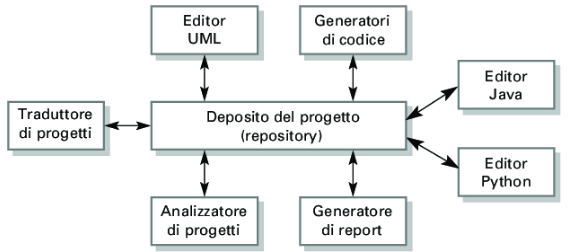
\includegraphics[width=0.8\linewidth]{figures/arch_repo.png}
      \end{figure}
      \subsubsection{Vantaggi}
        \begin{itemize}
            \item Possibile indipendenza tra i componenti (non devono trasmettere dati direttamente tra loro e non devono per forza sapere dell'esistenza degli altri);
            \item Repo gestisce tutti i dati concorrentemente (controllo accessi / backup);
            \item Semplice integrazione di nuovi componenti che si conformano al modello dati condiviso
        \end{itemize}
      \subsubsection{Svantaggi}
        \begin{itemize}
            \item Rende difficile la distribuzione su più macchine (ridondanza e inconsistenza a causa del dover mantenere coerenti / aggiornate copie degli stessi dati);
            \item Repository è \textbf{single point of failure} (tutti suoi problemi influiscono su tutto il sistema);
            \item Difficile integrazione di componenti non conformi al modello dati comune.
        \end{itemize}
    \subsection{Pattern client-server}
      Architettura \textbf{distribuita} in cui ciascun servizio viene fornito da un server separato al cui i client accedomo per utilizzarne i servizi.
      \begin{figure}[htpb]
          \centering
          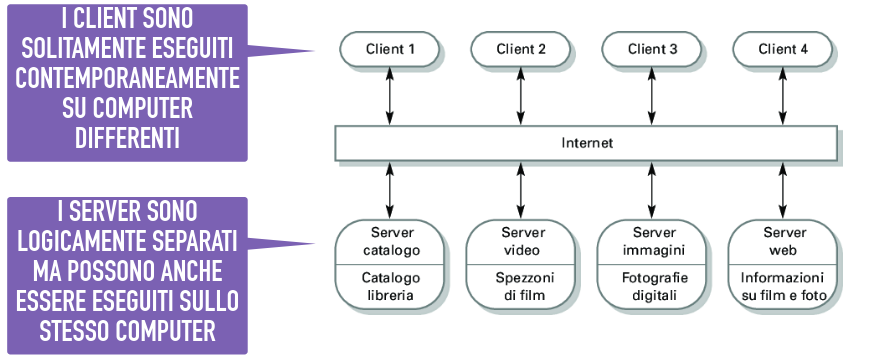
\includegraphics[width=0.8\linewidth]{figures/arch_cl_se.png}
      \end{figure}
      \subsubsection{Vantaggi}
        \begin{itemize}
            \item Server possono essere distribuiti su una rete;
            \item Server e servizi sono indipendenti / possono essere modificati senza intaccare altre parti del sistema;
            \item Facile aggiunta / integrazione di nuovi server al sistema.
        \end{itemize}
      \subsubsection{Svantaggi}
        \begin{itemize}
            \item Ciascun servizio costituisce un \textbf{single point of failure}, ma potrebbe essere replicato su più server;
            \item Prestazioni potrebbero dipendere da canali di comunicazione (congestione rete);
            \item Possibili problemi di gestione in caso di server proprietari di organizzazioni diverse.
        \end{itemize}
      \subsubsection{Componenti}
        Ogni applicazione viene suddivisa logicamente in 3 parti:
        \begin{itemize}
            \item \textbf{Presentazione} - gestione UI (eventi grafici, controlli su input...);
            \item \textbf{Logica applicativa} - logica e regole che definiscono elaborazione dei dati per rispondere alle richieste utente;
            \item \textbf{Gestione dei dati persistenti} - memorizzazione / gestione dei dati a lungo termine.
        \end{itemize}
        La distribuzione fisico-logica di queste componenti porta a classficazione delle architetture:
        \begin{itemize}
            \item \textbf{2-Tier}: suddivisa in \textit{client} e \textit{server}, la logica applicativa può essere distribuita tra i due;
            \item \textbf{3-Tier}: i tre livelli sono separati -> presentazione su \textit{client}, logica applicativa su un \textit{application server} e gestione dei dati su un \textit{database server} (scelta tipica per app web scalabili);
            \item \textbf{n-Tier}: utilizza ulteriori divisioni logico-fisiche aggiungendo livelli come \textit{Cache Layer} per ottimizzare prestazioni e \textit{Security Layer} per autenticazioni / autorizzazioni centralizzate (ideale per sistemi complessi - microservizi o app su cloud).
        \end{itemize}
      \subsubsection{Esempi}
        \noindent
          \begin{minipage}[c]{0.48\linewidth}
              \centering
              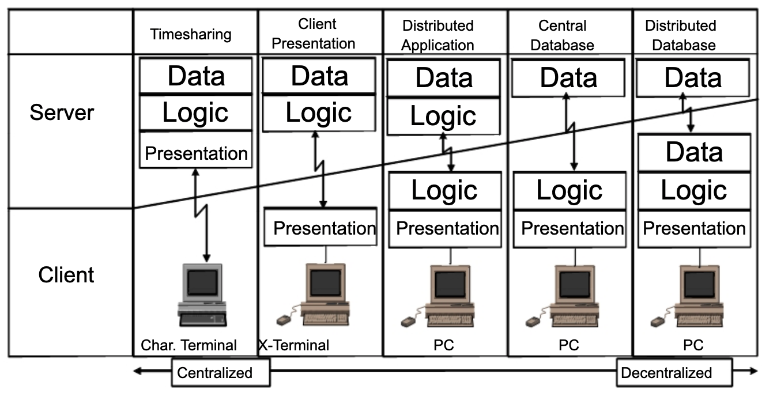
\includegraphics[width=0.8\linewidth]{figures/arch_cl_se_2.png}

              \captionof{figure}{Esempio 2-Tier}
          \end{minipage}
          \hfill
          \begin{minipage}[c]{0.48\linewidth}
              \centering
              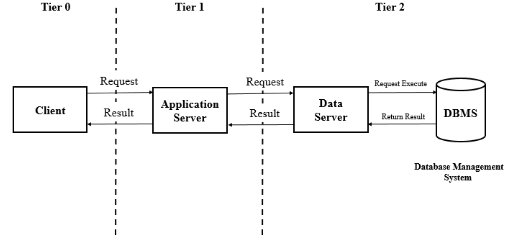
\includegraphics[width=0.8\linewidth]{figures/arch_cl_se_3.png}

              \captionof{figure}{Esempio 3-Tier}
          \end{minipage}
    \subsection{Pattern pipe-and-filter}
      Ciascun componente di elaborazione (filtro) è discreto e fornisce un output effettuando una trasformazione (in sequenza o in parallelo) dei dati in input. I dati fluiscono (singoli o in batch) attraverso una sequenza di componenti per essere elaborati.
      \begin{figure}[htpb]
          \centering
          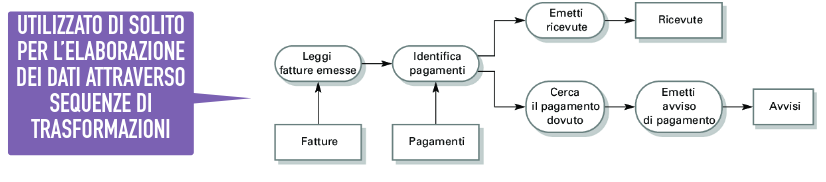
\includegraphics[width=0.8\linewidth]{figures/arch_bat.png}
      \end{figure}
      \subsubsection{Vantaggi}
        \begin{itemize}
            \item Evoluzione del sistema semplice mediante modifica / aggiunta di trasformazioni;
            \item Possibile riutilizzo trasformazioni;
            \item Possibile progettare separatamente componenti.
        \end{itemize}
      \subsubsection{Svantaggi}
        \begin{itemize}
            \item Trasformazioni successive devono rispettare formato concordato per trasferimento dati;
            \item Possibile non poter riusare componenti dati incompatibili / introdurre overhead per traduzione formato;
            \item Interazione con utenti limitata (interfacce con utenti solitamente non forniscono input come semplici flussi sequenziali continui).
        \end{itemize}
    \subsection{Pattern model-view-controller (MVC)}
      \noindent
        \begin{minipage}[c]{0.58\linewidth}
            Nasce da necessità di visualizzare dati generici mediante GUI usando rappresentazioni diverse, consente realizzazione di architettura che permette separazione dei componenti di presentazione da quelli che gestiscono i dati.
        \end{minipage}
        \hfill
        \begin{minipage}[c]{0.38\linewidth}
            \centering
            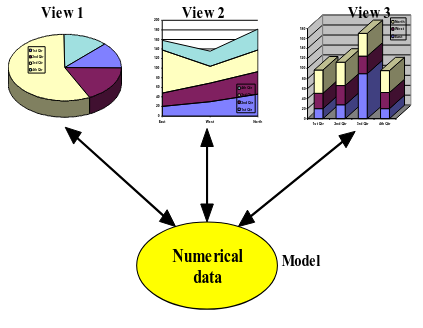
\includegraphics[width=0.8\linewidth]{figures/arch_mvc_1.png}
        \end{minipage}
      \begin{itemize}
          \item \textbf{model} contiene classi in cui istanze rappresentano dati da visualizzare / manipolare (forniscono anche i metodi per fare ciò);
          \item \textbf{view} contiene oggetti per presentare dati contenuti nel \textit{model} all'utente;
          \item \textbf{controller} contiene oggetti che controllano / gestiscono interazione dell'utente con \textit{view} e \textit{model}.
      \end{itemize}
      \begin{figure}[htpb]
          \centering
          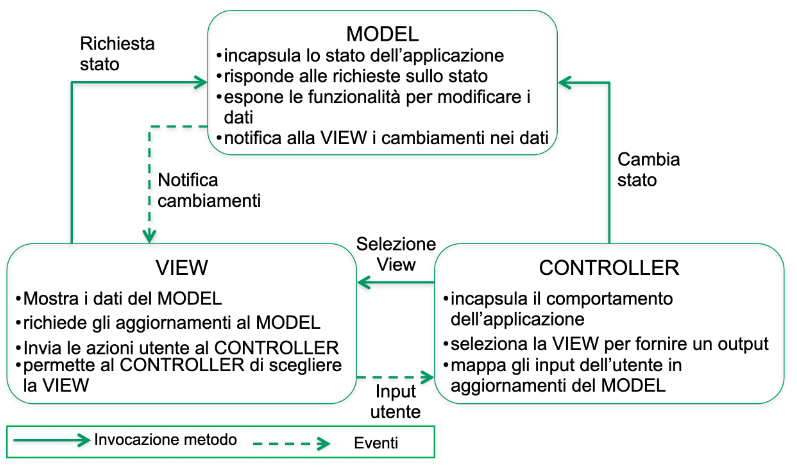
\includegraphics[width=0.6\linewidth]{figures/arch_mvc_2.png}
      \end{figure}
      \subsubsection{Aggiornamento dati}
        \begin{enumerate}
            \item In risposta a evento x il metodo \textbf{handleEvent()} viene invocato sul \textit{Controller};
            \item \textit{Controller} esamina stato di \textit{Model} e invoca suo metodo per cambiare il suo stato (\textbf{changeState()});
            \item \textit{Model} cambia lo stato e notifica lo notifica a tute le \textit{View} registrate (\textbf{notify()});
            \item Ogni \textit{View} registrata viene notificaa invocando suo metodo \textbf{update()}, la \textit{View} esamina lo stato di \textit{Model} mediante metodo \textbf{getState()}.
        \end{enumerate}
        \begin{figure}[H]
            \centering
            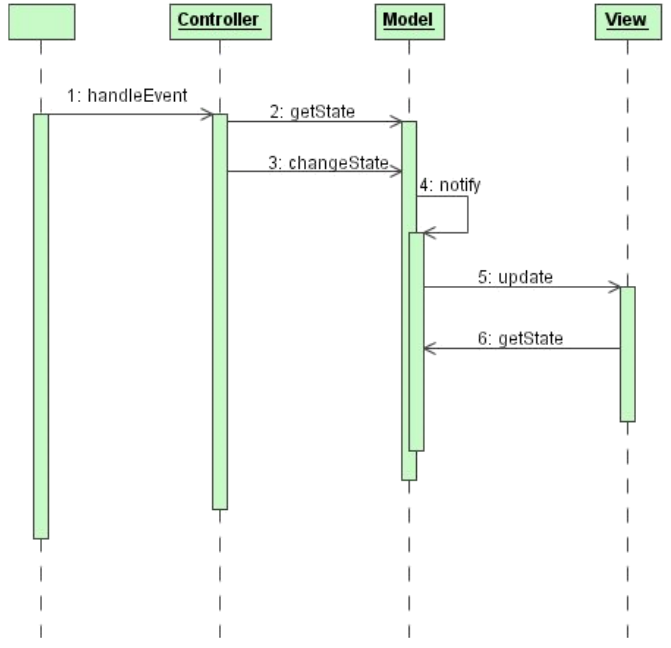
\includegraphics[width=0.4\linewidth]{figures/arch_mvc_ag.png}
        \end{figure}
      \subsubsection{Selezione schermata}
        \begin{enumerate}
            \item Utente seleziona una pagina da mostrare mediante \textit{View};
            \item \textit{View} delega a \textit{Controller} tramite invocazione del suo metodo \textbf{processSelectPage()};
            \item \textit{Controller} decide e/o compone pagina da visualizzare, comunicandola poi a \textit{View} invocando suo metodo \textbf{showSelectPage()};
            \item \textit{View} costruisce e presenta all'utente la schermata richiesta, con eventuale controllo su possibili modifiche in \textit{Model} invocando metodo \textbf{getState()}.
        \end{enumerate}
        \begin{figure}[H]
            \centering
            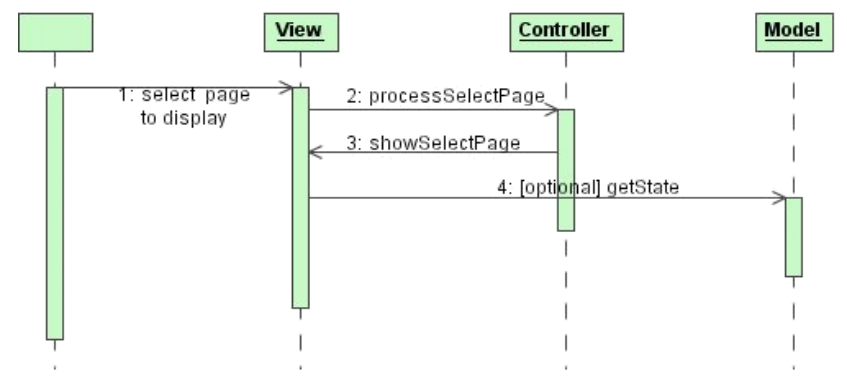
\includegraphics[width=0.6\linewidth]{figures/arch_mvc_sel.png}
        \end{figure}
\end{document}
